\documentclass[conference]{IEEEtran}
%\documentclass[onecolumn,draftcls]{IEEEtran}

\renewcommand\IEEEkeywordsname{Index Terms}

\usepackage{cite}

\usepackage[pdftex]{graphicx}
\graphicspath{{Figures/}}
\DeclareGraphicsExtensions{.pdf,.jpeg,.png}

\usepackage{amsmath}
\usepackage{tcolorbox}
\usepackage{subcaption}
\usepackage{amsfonts}
\usepackage{bbm}
\usepackage{url}
\usepackage{cleveref}

% Start \widebar implementation
\makeatletter
\let\save@mathaccent\mathaccent
\newcommand*\if@single[3]{%
  \setbox0\hbox{${\mathaccent"0362{#1}}^H$}%
  \setbox2\hbox{${\mathaccent"0362{\kern0pt#1}}^H$}%
  \ifdim\ht0=\ht2 #3\else #2\fi
  }
%The bar will be moved to the right by a half of \macc@kerna, which is computed by amsmath:
\newcommand*\rel@kern[1]{\kern#1\dimexpr\macc@kerna}
%If there's a superscript following the bar, then no negative kern may follow the bar;
%an additional {} makes sure that the superscript is high enough in this case:
\newcommand*\widebar[1]{\@ifnextchar^{{\wide@bar{#1}{0}}}{\wide@bar{#1}{1}}}
%Use a separate algorithm for single symbols:
\newcommand*\wide@bar[2]{\if@single{#1}{\wide@bar@{#1}{#2}{1}}{\wide@bar@{#1}{#2}{2}}}
\newcommand*\wide@bar@[3]{%
  \begingroup
  \def\mathaccent##1##2{%
%Enable nesting of accents:
    \let\mathaccent\save@mathaccent
%If there's more than a single symbol, use the first character instead (see below):
    \if#32 \let\macc@nucleus\first@char \fi
%Determine the italic correction:
    \setbox\z@\hbox{$\macc@style{\macc@nucleus}_{}$}%
    \setbox\tw@\hbox{$\macc@style{\macc@nucleus}{}_{}$}%
    \dimen@\wd\tw@
    \advance\dimen@-\wd\z@
%Now \dimen@ is the italic correction of the symbol.
    \divide\dimen@ 3
    \@tempdima\wd\tw@
    \advance\@tempdima-\scriptspace
%Now \@tempdima is the width of the symbol.
    \divide\@tempdima 10
    \advance\dimen@-\@tempdima
%Now \dimen@ = (italic correction / 3) - (Breite / 10)
    \ifdim\dimen@>\z@ \dimen@0pt\fi
%The bar will be shortened in the case \dimen@<0 !
    \rel@kern{0.6}\kern-\dimen@
    \if#31
      \overline{\rel@kern{-0.6}\kern\dimen@\macc@nucleus\rel@kern{0.4}\kern\dimen@}%
      \advance\dimen@0.4\dimexpr\macc@kerna
%Place the combined final kern (-\dimen@) if it is >0 or if a superscript follows:
      \let\final@kern#2%
      \ifdim\dimen@<\z@ \let\final@kern1\fi
      \if\final@kern1 \kern-\dimen@\fi
    \else
      \overline{\rel@kern{-0.6}\kern\dimen@#1}%
    \fi
  }%
  \macc@depth\@ne
  \let\math@bgroup\@empty \let\math@egroup\macc@set@skewchar
  \mathsurround\z@ \frozen@everymath{\mathgroup\macc@group\relax}%
  \macc@set@skewchar\relax
  \let\mathaccentV\macc@nested@a
%The following initialises \macc@kerna and calls \mathaccent:
  \if#31
    \macc@nested@a\relax111{#1}%
  \else
%If the argument consists of more than one symbol, and if the first token is
%a letter, use that letter for the computations:
    \def\gobble@till@marker##1\endmarker{}%
    \futurelet\first@char\gobble@till@marker#1\endmarker
    \ifcat\noexpand\first@char A\else
      \def\first@char{}%
    \fi
    \macc@nested@a\relax111{\first@char}%
  \fi
  \endgroup
}
% End \widebar implementation

\newcommand\defeq{\mathrel{\overset{\makebox[0pt]{\mbox{\normalfont\tiny\sffamily def}}}{=}}}
\newcommand{\ind}[1]{\mathbbm{1}_{\left\{ #1 \right\}}}
\newcommand*\mean[1]{\widebar{#1}}

\DeclareMathOperator*{\argmin}{minimize}
\DeclareMathOperator*{\argmax}{maximize}
\DeclareMathOperator{\sinc}{sinc}
\DeclareMathOperator{\var}{Var}

% correct bad hyphenation here
\hyphenation{net-works}

\setlength{\columnsep}{0.22in}

\begin{document}
\title{Joint Base Station Selection and Adaptive Slicing in Virtualized Wireless Networks:\\A Stochastic Optimization Framework}

\author{
\IEEEauthorblockN{Kory Teague$^1$, Mohammad J. Abdel-Rahman$^{1,2}$, and Allen B. MacKenzie$^1$\\}
\IEEEauthorblockA{$^1$Department of Electrical and Computer Engineering, Virginia Tech, Blacksburg, VA 24061, USA \\ $^2$Department of Electrical and Energy Engineering, Al Hussein Technical University (HTU), Amman 11821, Jordan \\
\{koryt, mo7ammad, mackenab\}@vt.edu
}}

\maketitle

\begin{abstract}
Wireless network virtualization is a promising avenue of research for next-generation 5G cellular networks.  Virtualization focuses on the concept of active resource sharing and the building of a network designed for specific demands, decreasing operational expenditures, and improving demand satisfaction of cellular networks.  This work investigates the problem of selecting base stations (BSs) to construct a virtual network that meets the the specific demands of a service provider, and adaptive slicing of the resources between the service provider's demand points.  A two-stage stochastic optimization framework is introduced to model the problem of joint BS selection and adaptive slicing.  Two methods were presented for determining an approximation for the two-stage stochastic optimization model.  The first method uses a sampling approach applied to the deterministic equivalent program of the stochastic model.  The second method uses a genetic algorithm for BS selection and adaptively slicing via a single-stage linear optimization problem.  For testing, a number of scenarios were generated using a log-normal model designed to emulate demand from real world cellular networks.  Our simulations indicate that the first approach can provide a reasonably tight solution, but is constrained as the time expense grows exponentially with the number of parameters.  The second approach provides a vast improvement in run time with the introduction of notable error.
\end{abstract}

\begin{IEEEkeywords}
Wireless network virtualization, resource allocation, two-stage stochastic optimization, genetic algorithm.
\end{IEEEkeywords}

\IEEEpeerreviewmaketitle



\section{Introduction} \label{sec:intro}

Wireless virtualization is one of the most promising approaches for efficient sharing of radio resources in next-generation mobile networks~\cite{6824752}.  In~\cite{6553675, 6571315}, the opportunities for cost saving and additional flexibility are the motivations behind introducing virtualization schemes for LTE networks, focusing on resource sharing.  Doyle et al.~\cite{6737248} presented the Network without Borders (NwoB) paradigm which broadly explores the concepts of virtualization.  The authors proposed removing the traditional constraints on spectrum and presented a virtualization-centric structure for mobile wireless networks.  In this paradigm, a service provider (SP) provides a specified service to its users, which could be in the form of traditional general data, voice, and messaging services or a more specific application (e.g., emergency services, Internet of things, or video streaming).  The virtual network builder (VNB) aggregates and selects resources from resource providers (RPs) to build virtual networks designed for the needs of the SPs.  RPs, such as traditional MNOs, are the owners and maintainers of the physical resources and infrastructure that are provided for the virtualized wireless networks (VWNs) via contracts established with VNBs.

Considering the uncertainty of user equipment (demand point) locations, in this paper we consider solving two problems jointly.  The first problem is to optimally orchestrate a set of BSs from a set of RPs to meet the demands of an SP.  The second problem is to slice the set of selected BSs adaptively between the demand points of the SP according to changes in distribution.  Stochastic programming provides a powerful mathematical tool to handle optimization under uncertainty.  It had been recently exploited to optimize resource allocation in various types of wireless networks operating under uncertainties (examples include~\cite{MJ_TW_13, CC_OFDMA, MJ_MECOMM_17, MJ_CCNC_16, MJ_WCNC_16, MJ_DySPAN_15, CC_video}).  We establish a stochastic optimization problem from the perspective of the VNB to jointly solve the problems.  Then, we develop two approaches that would be run in the VNB to reach a near-optimal solution of the stochastic optimization problem.  We consider two optimality criteria: maximizing demand satisfaction of SP users and minimizing the cost of network construction.  Finally, we consider the efficacy of the approaches with a single SP with log-normal spatially-correlated demand modeled to mimic real cellular networks.

The rest of this paper is organized as follows.  \Cref{sec:model} details and defines the system model assumed for this paper.  \Cref{sec:approach} establishes our stochastic optimization problem and approximation approaches.  \Cref{sec:sim} simulates the approaches and evaluates their performance.  \Cref{sec:conclusion} discusses our conclusions and directions of future research.

\section{System Model} \label{sec:model}

We consider a geographic region, $\mathcal{R}$, of width $X$ (m) and length $Y$ (m) that contains a VNB and a set $\mathcal{S} \defeq \left\{ 1,\, 2,\, \ldots,\, S \right\}$ of virtualized BSs the VNB had aggregated for use from a set of RPs.  The rate capacity of BS $s \in \mathcal{S}$ is denoted by $r_s$, its cost $c_s$, and its coverage radius $b_s$.

An SP seeking a VWN from the VNB is assumed to know the distribution of traffic demand within the region the VWN would cover.  It has been shown that a log-normal distribution or a mixture of log-normal distributions can approximate traffic demand in real-world cellular networks~\cite{686105, 5936263}.  It has also been shown that traffic distribution is spatially correlated~\cite{5936263, eigenplaces}.  We model the spatial traffic demand of a single SP using a similar, continuous form of the SSLT (Scalable, Spatially-correlated, and Log-normally distributed Traffic) model as proposed by Lee, Zhou, and Niu~\cite{6554749}.  Our implementation differs from theirs by converting the SSLT model into a continuous, not pixelated, form.  This continuous SSLT is denoted as $\lambda \left( x,\, y \right)$.

Let $\mathcal{M} \defeq \left\{ 1,\, 2,\, \ldots,\, M \right\}$ be the set of the SP's demand points seeking to connect to the VWN; the traffic demand at each point is denoted by $d_m$.  Let $u_{ms} \in \left[ 0,\, 1 \right],\, m \in \mathcal{M},\, s \in \mathcal{S}$, represent the normalized maximum rate (with respect to $r_s$) that a user at point $m$ can receive from BS $s$.  $u_{ms} = 0$ when $m$ is outside the coverage area of $s$ and $u_{ms} = 1$ otherwise.  The specific position of the points in $\mathcal{M}$, and therefore the values of $u_{ms}$, is determined via a non-stationary 2D Poisson point process (PPP) with $M$ points using the demand field, $\lambda \left( x,\, y \right)$, as the spatial intensity function.  To generate this non-stationary PPP, we use an accept-reject method~\cite{leeds:nsPPPgeneration}.

We assume that a BS $s \in \mathcal{S}$ can be allocated between multiple demand points, and $\delta_{ms} \in \left[ 0,\, r_s \right],\, m \in \mathcal{M},\, s \in \mathcal{S}$, represents the rate of BS $s$ that is allocated to point $m$.

\section{Solution Approach} \label{sec:approach}

In this section, we detail our approaches for selecting resources within $\mathcal{S}$ to construct a VWN.  First, we formulate the problem as a two-stage stochastic optimization program.  Second, the optimization problem is converted to its deterministic equivalent program and sampled.  Finally, a genetic algorithm is used as an approximation of BS selection.

\subsection{Problem Formulation} \label{subsec:stoch}

\begin{tcolorbox}[floatplacement = !ht, float, title = Problem 1:\\Two-Stage Stochastic Optimization Program]
\begin{align}
& \argmin_{\left\{ z_s \right\}} \left\{ \sum_{s \in \mathcal{S}} c_s \; z_s - \alpha \; \mathbb{E}\left[ h\left( \textit{\textbf{z}},\, \tilde{\textit{\textbf{u}}} \right) \right] \right\} \label{eq:SOPS1O}\\
& \text{subject to:}  \nonumber \\
& \hspace{0.4in} z_s \in \left\{ 0,\, 1 \right\},\, \forall s \in \mathcal{S} \label{eq:SOPS1C1}
\end{align}
where $h(\textit{\textbf{z}}, \tilde{\textit{\textbf{u}}})$ is the optimal value of the second-stage problem, which is given by:
\begin{align}
& \argmax_{\left\{ \delta_{ms} \right\}} \left\{ \sum_{m \in \mathcal{M}} \sum_{s \in \mathcal{S}} \delta_{ms} \; \tilde{u}_{ms} \right\} \label{eq:SOPS2O}\\
& \text{subject to:}  \nonumber \\
& \hspace{0.4in} z_s = \ind{\sum_{m \in \mathcal{M}} \delta_{ms} > 0},\, \forall s \in \mathcal{S} \label{eq:SOPS2C1}\\
& \hspace{0.4in} \sum_{s \in \mathcal{S}} \delta_{ms} \; \tilde{u}_{ms} \leq d_m,\, \forall m \in \mathcal{M} \label{eq:SOPS2C2}\\
& \hspace{0.4in} \sum_{m \in \mathcal{M}} \delta_{ms} \leq r_s,\, \forall s \in \mathcal{S} \label{eq:SOPS2C3}\\
& \hspace{0.4in} \delta_{ms} \in \left[ 0,\, d_m \right],\, \forall m \in \mathcal{M},\, \forall s \in \mathcal{S} \label{eq:SOPS2C4}
\end{align}
\end{tcolorbox}

To formulate the presented problem, we introduce $z_s,\, s \in \mathcal{S}$, as a binary decision variable defined such that $z_s = 1$ if BS $s$ is selected for the created VWN and $z_s = 0$ otherwise.  To balance maximizing demand satisfaction against minimizing cost, we introduce positive real number $\alpha$ as a weighting coefficient.

The first stage objective function (\cref{eq:SOPS1O}) minimizes the total cost of the selected network with respect to that network's ability to satisfy the demand contained within the region.  The second stage objective function (\cref{eq:SOPS2O}) maximizes demand satisfaction by maximizing the total demand allocated to the resources comprising the network, as specified by $\delta_{ms}$ as the decision variable of the second stage.

\Cref{eq:SOPS2C1} ensures that demand is allocated only to selected resources; $\mathbbm{1}_{\left\{ * \right\}}$ is the indicator function defined such that $\mathbbm{1}_{\left\{ * \right\}} = 1$ if condition $\left\{ * \right\}$ is true and $\mathbbm{1}_{\left\{ * \right\}} = 0$ otherwise.  \Cref{eq:SOPS2C2} ensures that demand points are not allocated more resources than demanded, and \cref{eq:SOPS2C3} ensures that BSs are not allocated more demand than can be satisfied.

\subsection{Deterministic Equivalent Reformulation} \label{subsec:dep}

To solve Problem 1, it is converted to a deterministic equivalent program (DEP) and does not contain any stochastic variables~\cite{stochprogramming}.  The DEP accounts for all realizations of the stochastic variables, converting them into a set of scenarios weighted by their probability.  However, this set of all scenarios is impractically large and must be sampled.

Let $\hat{\Omega} \defeq \left\{ 1,\, 2,\, \ldots, O \right\}$ be this set of sampled scenarios.  Each scenario $\omega \in \hat{\Omega}$ is defined by $u_{ms}^{\left( \omega \right)}$ generated from a single, independent realization of demand points according to $\lambda\left( x,\, y \right)$.  Due to this independent sampling, each scenario in $\hat{\Omega}$ has equal probability, $\frac{1}{O}$.  Substituting the stochastic variables for the set of deterministic scenarios converts Problem 1 into its sampled DEP (sDEP) formulation.

\begin{tcolorbox}[floatplacement = !ht, float, title = Problem 2: Sampled DEP (sDEP)]
\begin{align}
& \argmin_{\left\{ z_s,\, \delta_{ms}^{\left( \omega \right)} \right\}} \left\{ \sum_{s \in \mathcal{S}} c_s \; z_s - \frac{\alpha}{O} \sum_{\omega \in \hat{\Omega}} \sum_{m \in \mathcal{M}} \sum_{s \in \mathcal{S}} \delta_{ms}^{\left( \omega \right)} \; u_{ms}^{\left( \omega \right)} \right\} \label{eq:sDEPO}\\
& \text{subject to:}  \nonumber \\
& \hspace{0.4in} \sum_{s \in \mathcal{S}} \delta_{ms}^{\left( \omega \right)} \; u_{ms}^{\left( \omega \right)} \leq d_m,\, \forall m \in \mathcal{M},\, \forall \omega \in \hat{\Omega} \label{eq:sDEPC1}\\
& \hspace{0.4in} \sum_{m \in \mathcal{M}} \delta_{ms}^{\left( \omega \right)} \leq r_s \; z_s,\, \forall s \in \mathcal{S},\, \forall \omega \in \hat{\Omega} \label{eq:sDEPC2}\\
& \hspace{0.4in} z_s \in \left\{ 0,\, 1 \right\},\, \forall s \in \mathcal{S}. \label{eq:sDEPC3}\\
& \hspace{0.4in} \delta_{ms}^{\left( \omega \right)} \in \left[ 0,\, d_m \right],\, \forall m \in \mathcal{M},\, \forall s \in \mathcal{S},\, \forall \omega \in \hat{\Omega} \label{eq:sDEPC4}
\end{align}
\end{tcolorbox}

The objective function (\cref{eq:sDEPO}) combines both objective functions of Problem 1.  \Cref{eq:sDEPC1,eq:sDEPC2} ensure demand is not overallocated and is only allocated to selected resources within those resources' capacities for all scenarios.

Problem 2 provides an equivalent deterministic form of Problem 1 for the sampled sample space, $\hat{\Omega}$.  With a sufficiently large $O$, $\hat{\Omega}$ approaches a tight approximation of the whole sample space at the cost of computational complexity.

\subsection{Adaptive Slicing within a Formed VWN} \label{subsec:slice}

After the solution to the sDEP has been found, the VNB has determined the joint BS selection that forms the VWN and a proposed resource slicing of considered possible scenarios, $\hat{\Omega}$, that allocates the resources to the SP's demand points.  After BS selection, any observed scenario is unlikely to be in $\hat{\Omega}$.  The VNB must adapt its resource slicing to the new realization.  The joint BS selection, $z_s$, becomes a constant of the network, simplifying Problem 2.

\begin{tcolorbox}[floatplacement = !ht, float, title = Problem 3: Adaptive Slicing Model]
\begin{align}
& \argmin_{\left\{ \delta_{ms} \right\}} \left\{ \sum_{m \in \mathcal{M}} \sum_{s \in \mathcal{S}} \delta_{ms} \; u_{ms} \right\} \label{eq:ASMO}\\
& \text{subject to:}  \nonumber \\
& \hspace{0.4in} \sum_{s \in \mathcal{S}} \delta_{ms} \; u_{ms} \leq d_m,\, \forall m \in \mathcal{M} \label{eq:ASMC1}\\
& \hspace{0.4in} \sum_{m \in \mathcal{M}} \delta_{ms} \leq r_s \; z_s,\, \forall s \in \mathcal{S}. \label{eq:ASMC2}\\
& \hspace{0.4in} \delta_{ms} \in \left[ 0,\, d_m \right],\, \forall m \in \mathcal{M},\, \forall s \in \mathcal{S} \label{eq:ASMC3}
\end{align}
\end{tcolorbox}

It is worth noting that Problem 3 is less computationally complex than Problem 2 as it only contains the single continuous decision variable for resource slicing, simplifying Problem 3 to a linear programming problem.

\subsection{Genetic Algorithm Approach} \label{subsec:ga}

The Problem 2 formulation becomes intractable as $O$, $S$, or $M$ increases.  Most importantly, the accuracy of the sDEP is directly dependent on the size of $\hat{\Omega}$, $O$, directly causing a trade off between the accuracy of the sDEP and its computability in a reasonable amount of time.  Through the less computationally complex Problem 3, an approximation of Problem 1 can be found by finding an optimal BS selection.  In this subsection, we reformulate the problem of joint BS selection for the VWN as a genetic algorithm (GA).

A GA is an iterative metaheuristic in which an approximate solution to a given optimization problem is arrived at via a series of progressive generations.  Each generation contains a number of candidate solutions (individuals), each defined by a chromosome.  Each individual is assessed by its fitness; the fitter an individual, the better its solution.  Then individuals are \emph{selected} at random, with more fit individuals being selected with higher probability.  Pairs of selected individuals will \emph{crossover} with probability $p_\text{xov}$, a process similar to genetic recombination in biology.  The resulting chromosomes then have probability $p_\text{mut}$ to \emph{mutate}, altering the chromosome slightly.  The resultant children individuals form the next generation, and the process repeats.

Let $\mathcal{G} \defeq \left\{1,\, 2,\, \ldots,\, G\right\}$ be the set of generations used in the GA and $\mathcal{I}_g \defeq \left\{1,\, 2,\, \ldots,\, I\right\}, g \in \mathcal{G}$ be the set of individuals within generation $g$.  Each individual $i \in \mathcal{I}_g$ has a binary chromosome $\textbf{z}^{\left\{ ig \right\}}$.  Each bit of $\textbf{z}^{\left\{ ig \right\}}$, $z_s^{\left\{ ig \right\}}, s \in \mathcal{S}$, is defined such that $z_s^{\left\{ ig \right\}} = 1$ if BS s is selected by individual $i$ in generation $g$ and $z_s^{\left\{ ig \right\}} = 0$ otherwise.

We assume that all demand over the region is allocated to the closest resource.  Let $\mathcal{S}^{\left\{ ig \right\}} \subseteq \mathcal{S}$ be the set of BSs selected by $\textbf{z}^{\left\{ ig \right\}}$.  The total demand allocated to BS $s \in \mathcal{S}^{\left\{ ig \right\}}$ is $\iint_{V_s} \lambda\left( x,\, y \right) \,dx \,dy$, where $V_s$ is the region bounded by the cell of BS $s$ in the Voronoi tessellation of $\mathcal{S}^{\left\{ ig \right\}}$.  If this allocated demand exceeds $r_s$, then BS $s$ is said to be \emph{overcapacity}.  Let $B_s$ be the region within the coverage radius of BS $s$.  If $V_s \not\subseteq B_s$, then BS $s$ is considered \emph{overcoverage}.

The fitness of each individual, $\textbf{z}^{\left\{ ig \right\}}$, is assessed as

\begin{equation} \label{eq:GAFit}
\text{fitness}\left( \textbf{z}^{\left\{ ig \right\}} \right) = \frac{1}{\text{cost}\left( \textbf{z}^{\left\{ ig \right\}} \right)}
\end{equation}
\begin{multline} \label{eq:GACost}
\mathrm{cost}\left( \textbf{z}^{\left\{ ig \right\}} \right) = \sum_{s \in \mathcal{S}} \Biggl( c_s \; z_s^{\left\{ ig \right\}} + c_\text{cov} \; \ind{V_s \not\subseteq B_s} + \\ \left( c_\text{cap}^g - 1 \right) \; \max\left( 0,\, \iint_{V_s} \lambda_n\left( x,\, y \right)\, dx\, dy - r_s \right) \Biggr)
\end{multline}

\noindent where cost is the sum of the cost of the resources and their overcoverage ($c_\text{cov}$) and overcapacity ($c_\text{cap}$) costs.  Overcoverage resources are not desired.  Overcapacity resources are allowed in early generations to increase exploration of the search space, but are trimmed as the overcapacity cost increases exponentially.

Elitism is used, where the $n$ fittest individuals of each generation are selected without crossover or mutation for the next generation.  Selection occurs via the roulette wheel selection method.  Every individual $i$ of generation $g$ has a selection probability of $\frac{\text{fitness}\left( \textbf{z}^{\left\{ ig \right\}} \right)}{\sum_{i \in \mathcal{I}} \text{fitness}\left( \textbf{z}^{\left\{ ig \right\}} \right)}$.

When crossover is performed on selected individuals, it is via the uniform crossover method with a mixing ratio of 0.5.  Mutation is bitwise, with each bit mutating (i.e., flipping) with probability $\frac{1}{S}$.  The uniqueness property is then enforced on the resulting children to ensure diversity; if a child chromosome is identical to another child chromosome in the next generation, the child is discarded and a new child generated.

The GA iterates for a number of generations $G$.  If it settles on a single individual for a number of continuous generations, $G_\text{halt}$, it will halt.  The chromosome of the fittest individual of the final generation determines $z_s$.  With this selection, the VNB then determines an adaptive slicing using Problem 3.

\section{Simulation and Evaluation} \label{sec:sim}

In this section, we evaluate the sDEP and GA approaches as approximations of Problem 1.  We will compare approach cost, demand satisfaction, and computation time.

\subsection{Setup} \label{subsec:setup}

\begin{table}
\vspace{0.1in}
\centering
\caption{Numerical Values of Relevant Parameters}
\begin{tabular}{|c|c|} 
\hline
Width, Height of Geographic Area & 2 km x 2 km \\
\hline
Number of BSs ($S$) & 60 \\ 
\hline 
Number of Demand Points ($M$) & 75 \\ 
\hline 
Number of Sampled Scenarios ($O$) & $\{5,\, 10,\, \ldots,\, 50\}$ \\ 
\hline 
BS cost ($c_s, \forall s \in \mathcal{S}$) & 1 \\ 
\hline 
BS capacity ($r_s, \forall s \in \mathcal{S})$ & 1.50 Mbps \\ 
\hline
BS range ($b_s, \forall s \in \mathcal{S}$) & 500 m \\
\hline 
Point Traffic Demand ($d_m, \forall m \in \mathcal{M}$) & 0.178 Mbps \\ 
\hline
Maximum Number of Generations ($G$) & 3000 \\ 
\hline
Minimum Number of Generations & 300 \\
\hline
Unchanged Generations Before Halt ($G_\text{halt}$) & 150 \\
\hline 
Number of Individuals per Generation ($I$) & 80 \\ 
\hline
Number of Elite Individuals per Generation & 4 \\
\hline 
Probability of Crossover ($p_\text{xov}$) & 0.7 \\ 
\hline 
Overcoverage Cost ($c_\text{cov}$) & 3 \\
\hline
Overcapacity Cost ($c_\text{cap}$) & 1.015 \\
\hline
\end{tabular}
\label{tab:simval}
\end{table}

\begin{figure*}[t]
	\centering
	\begin{minipage}{0.64\textwidth}
		\begin{subfigure}{.48\textwidth}
			\centering
			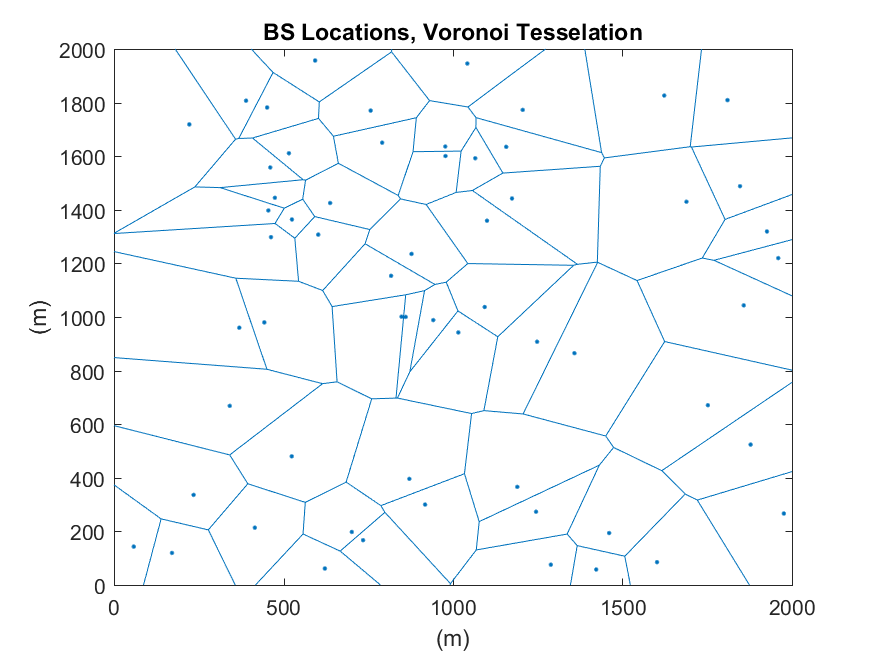
\includegraphics[width=0.95\linewidth]{Figures/BSLocationsVoronoi}
			\caption{Voronoi tesselation of BS locations}
			\label{fig:BSLocVor}
		\end{subfigure} \hfill
		\begin{subfigure}{.48\textwidth}
			\centering
			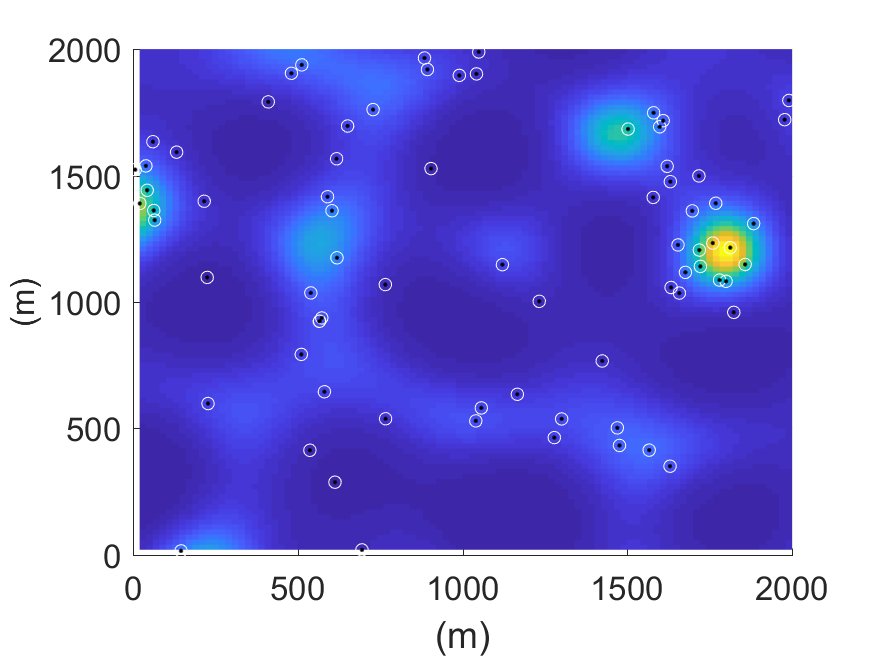
\includegraphics[width=0.95\linewidth]{Figures/SSLTnsPPP_demandpointreal}
			\caption{$\lambda$ with one realization of $\mathcal{M}$}
			\label{fig:SSLTDPReal}
		\end{subfigure}
		\caption{\small Visualization of resources (\cref{fig:BSLocVor}) and demand (\cref{fig:SSLTDPReal}) in $\mathcal{R}$.}
		\label{fig:NetworkArea}
	\end{minipage} \hfill
	\begin{minipage}{0.32\textwidth}
		\centering
		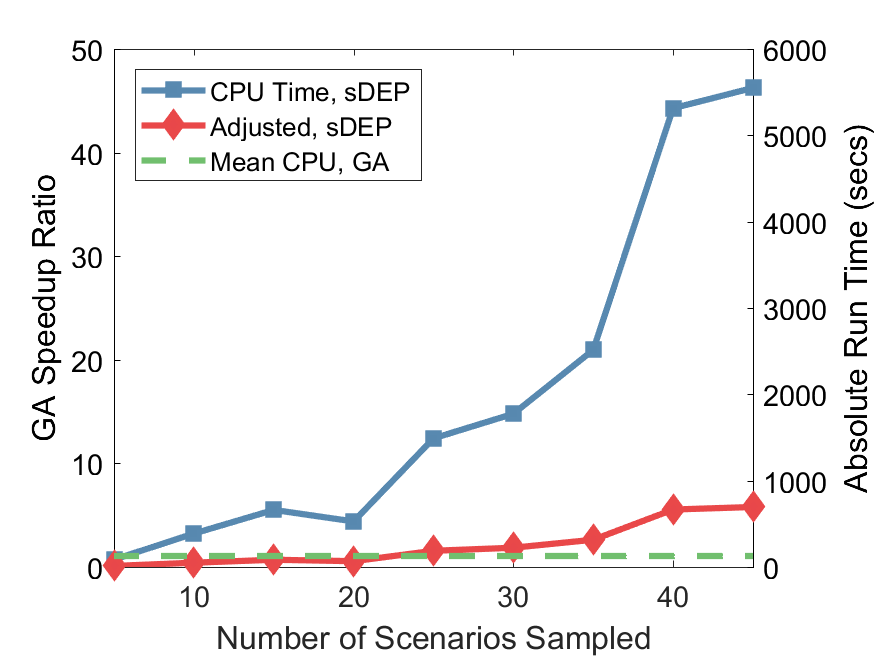
\includegraphics[width=0.95\textwidth]{Figures/VOSGA_SpeedupRatio_AbsComp_alpha20}
		\caption{\small Absolute run time and speedup ratio of the GA and sDEP approaches. $\alpha = 20$}
		\label{fig:AlgSpeedupRunTime}
	\end{minipage}
\end{figure*}

Simulation parameters are shown in \Cref{tab:simval}.  \Cref{fig:NetworkArea} provides a visualization of the simulation network area.  \Cref{fig:BSLocVor} shows the BS locations of $\mathcal{S}$ with the associated Voronoi tessellation showing the coverage areas of the BSs when all are active.  \Cref{fig:SSLTDPReal} shows the SSLT demand density field with one example scenario of demand points.  To compute the integral of the fitness function (\cref{eq:GACost}), $\lambda\left( x,\, y \right)$ is pixellated with the demands of all pixels within a Voronoi cell summed.

We ran our simulations on an Intel Core i7-4790K 4 GHz 4 core/8 thread CPU with 16 GB of DDR3 RAM.  We used CPLEX~\cite{Cplex} to solve Problems 2 and 3, and we used MATLAB to simulate the GA.  During simulations, extraneous processes were culled to allow maximal use of computer resources.  Average values for the performance of the genetic algorithm are provided from 50 independent runs using identical data except for the GA's initial set of individuals.

\subsection{Results} \label{subsec:results}

\Cref{fig:AlgSpeedupRunTime} shows a comparison of the approach run times in terms of the GA speedup ratio and CPU time.  As the number of scenarios sampled increases, the CPU run time of the sDEP increases exponentionally, and fails to converge to a final solution with 50 scenarios within the time limit of 15 minutes.  The GA converges to a solution in less CPU time than the sDEP.  The GA has a speedup ratio of 4.4x when the sDEP samples 20 scenarios; this increases to 46.3x with 45 scenarios.  A comparison of ``wall clock'' run times can be estimated by accounting for CPLEX's 8 thread parallel processing.  In terms of the adjusted approximate ``wall clock" time, the genetic algorithm converges in less wall clock time than the sDEP for 25 or more sampled scenarios.

\begin{figure*}[t]
\centering
\begin{subfigure}{.3\textwidth}
	\centering
	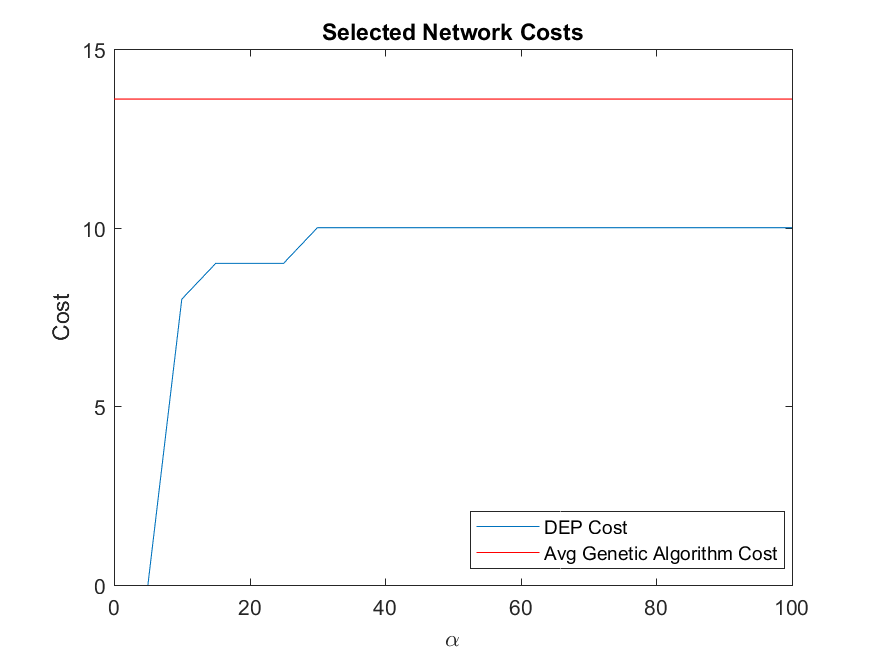
\includegraphics[width=1\linewidth]{Figures/ComparisonCost}
	\caption{VWN costs}
	\label{fig:VWNCompCost}
\end{subfigure}
\hspace{0.3cm}
\begin{subfigure}{.3\textwidth}
	\centering
	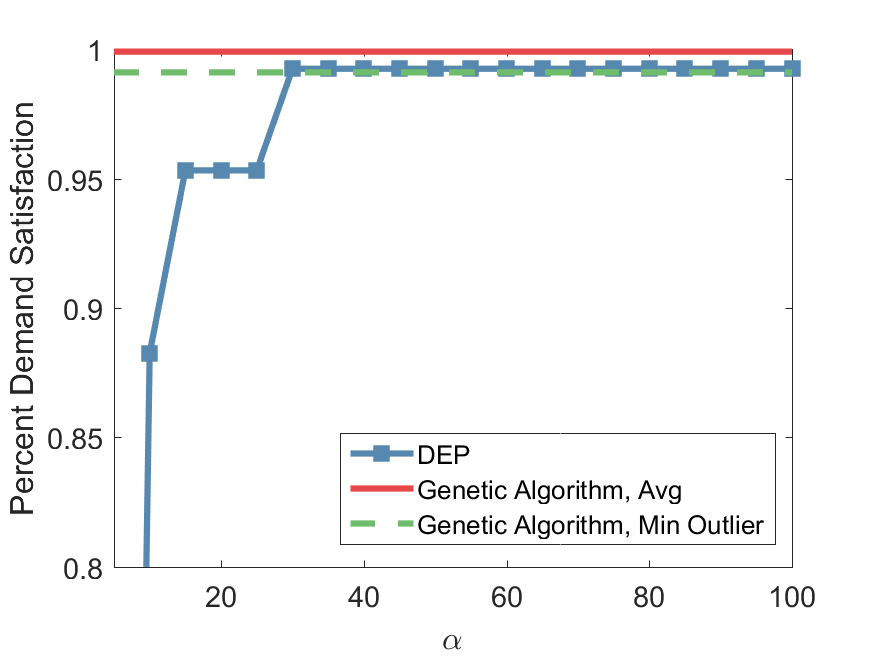
\includegraphics[width=1\linewidth]{Figures/ComparisonSatisfaction}
	\caption{SP demand point satisfaction}
	\label{fig:VWNCompSatis}
\end{subfigure}
\hspace{0.3cm}
\begin{subfigure}{.3\textwidth}
	\centering
	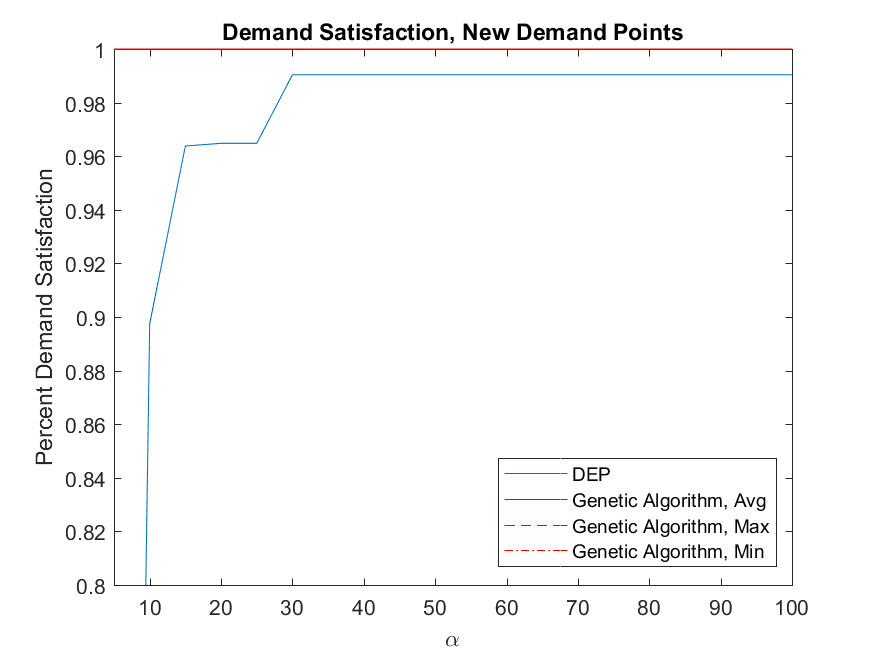
\includegraphics[width=1\linewidth]{Figures/ComparisonSatisfactionEval}
	\caption{50 new scenarios of 200 SP demand points evalutaed with Problem 3.}
	\label{fig:VWNCompSatisEval}
\end{subfigure}
\caption{\small Comparison of VWN costs and SP demand point satisfaction.}
\label{fig:VWNComp}
\end{figure*}

The GA's improved run time is at the expense of the accuracy of the solution.  \Cref{fig:VWNCompCost} compares the increasing cost of the sDEP to the GA as $\alpha$ increases.  On average, the GA incurs a 36\% increased cost in selecting the BSs for the VWN; at minimum, 20\%.  It should also be noted that the minimum quanta is 1 BS or 10\% additional cost for $\alpha \geq 30$, implying this increased cost could be overstated.  Increasing the number of BSs that construct the VWN would introduce additional granularity and might decrease this inefficiency.

There is a direct correlation between the number of selected BSs in the VWN and its demand satisfaction.  As the number of BSs selected (i.e., cost) increases, the average demand satisfaction approaches 100\%, as shown in \Cref{fig:VWNCompSatis}.  Because of overallocation, GA solutions average 99.9\% demand satisfaction.  The 10-BS sDEP solutions average 99.2\% when slicing to the scenarios in $\hat{\Omega}$, for which it is optimized.

When the demand points change to a scenario no longer in $\hat{\Omega}$, the sDEP performs similarly but less effectively.  \Cref{fig:VWNCompSatisEval} shows the demand satisfaction for both the sDEP and GA BS selections when sliced to 50 new scenarios not in $\hat{\Omega}$.  Each scenario contains 200 demand points demanding 66.8 kbps.  The demand satisfaction trend of the sDEP BS selection follows closely to before but hits a maximum of 99.0\% demand satisfaction with 10 BSs.  In comparison, the GA reaches $> 99.99\%$ demand satisfaction for all VWN scenarios.  This is expected as the increased number of points and scenarios more accurately describes the original SSLT demand density field, $\lambda$.

\section{Conclusion} \label{sec:conclusion}

In this work, we studied the problem of determining the optimal joint BS selection for a VWN and adaptively slicing the network to SP demand points.  We introduced a two-stage stochastic optimization problem which minimizes the cost of BS selection while maximizing network demand satisfaction.  We then investigated two approaches that provide an approximation for the model: a sampled deterministic equivalent program and a genetic algorithm that determines BS selection that is sliced via a single-stage optimization problem.

The first provides a tight approximate solution to the original stochastic model according to the number of sampled scenarios.  However, it is time prohibitive to converge to a solution as larger sets of resources and demand points are considered.  The second is a hybrid approach intending to simplify the first stage of the model in which all demand is allocated to the closest resource.  This approach simplifies the original model to a single-stage model which slices demand points to the GA's selected BSs.  This provides a faster solution with the introduction of error.

The simulation results indicate that the GA may be an adequate avenue for a solution.  This approach trends to a solution in 2\% of the time, incurring 20\% increased cost.  While the error is significant, it could decrease with larger data sets that would provide more resolution.  Increasing the size of the data set incurs a larger time cost on the sDEP than on the GA.  Analyzing these larger data sets or utilizing other metaheuristic algorithms would be obvious avenues for further investigation.

\bibliography{GenAlg_VWN-KTeag}
\bibliographystyle{IEEEtran}

\end{document}
